

\section{Giải pháp đề xuất}

\textit{Chương 3 của luận văn tập trung vào việc đề xuất giải pháp thay thế hệ thống quản lý cơ sở dữ liệu hiện tại là MSSQL bằng Greenplum. Đầu tiên, chương này trình bày các bước cần thiết để chuyển đổi từ MSSQL sang cơ sở dữ liệu phân tán, bao gồm phân tích các yêu cầu, lựa chọn công cụ hỗ trợ, và các thách thức có thể gặp phải trong quá trình chuyển đổi.}

\textit{Tiếp theo, chương này đi sâu vào quá trình lựa chọn Greenplum như là giải pháp thay thế cho MSSQL. Các tiêu chí lựa chọn bao gồm khả năng mở rộng, tính tương thích với hệ thống hiện tại, và khả năng xử lý dữ liệu lớn. Chương này cũng phân tích lý do tại sao Greenplum, với kiến trúc MPP (Massively Parallel Processing), lại phù hợp với yêu cầu của hệ thống ASP.NET Membership, đặc biệt là trong việc xử lý các tác vụ liên quan đến dữ liệu lớn và tối ưu hóa hiệu suất truy vấn.}

\textit{Cuối cùng, chương 3 đề cập đến quá trình chuẩn bị và triển khai Greenplum trong môi trường thử nghiệm, bao gồm việc cài đặt, cấu hình, và tích hợp với hệ thống hiện tại. Chương này cũng nhấn mạnh các kết quả ban đầu và những lợi ích mà Greenplum mang lại, như tăng cường hiệu suất xử lý và giảm thiểu thời gian truy vấn, từ đó giúp hệ thống đáp ứng tốt hơn các yêu cầu về khả năng mở rộng và hiệu suất.}

Trong thời đại kỹ thuật số hiện nay, việc quản lý và xử lý hiệu quả lượng dữ liệu ngày càng tăng trong các hệ thống thông tin là cực kỳ quan trọng. Các hệ thống cơ sở dữ liệu truyền thống như MSSQL đã chứng minh được nhiều giá trị, nhưng cũng bộc lộ những hạn chế nghiêm trọng trong việc đáp ứng nhu cầu về hiệu suất cao và khả năng mở rộng trong quản lý dữ liệu lớn. Như đã phân tích trong chương \ref{sec:introduction}, các vấn đề như tốc độ truy vấn chậm, quản lý tài nguyên không hiệu quả, và hạn chế về khả năng mở đã làm suy giảm hiệu suất của các hệ thống quản lý thành viên trực tuyến như ASP.NET Membership database. Để giải quyết những vấn đề này sẽ đề xuất việc chuyển đổi cơ sở dữ liệu ASP.NET Membership từ MSSQL sang một hệ thống cơ sở dữ liệu phân tán.

\subsection{Chuyển đổi MSSQL sang cơ sở dữ liệu phân tán}

Việc chuyển đổi cơ sở dữ liệu ASP.NET Membership từ một hệ thống cơ sở dữ liệu tập trung như MSSQL sang một hệ thống cơ sở dữ liệu phân tán đòi hỏi phải thực hiện một loạt các bước kỹ thuật chi tiết. Quá trình này không chỉ bao gồm việc di chuyển dữ liệu mà còn phải đảm bảo rằng tất cả các chức năng và hiệu suất của hệ thống được duy trì hoặc cải thiện. Dưới đây là các bước chi tiết để thiết lập hệ thống cơ sở dữ liệu phân tán phù hợp cho ASP.NET Membership Database.

\subsubsection{Kiến trúc lược đồ cơ sở dữ liệu}

\begin{figure}
    \centering
    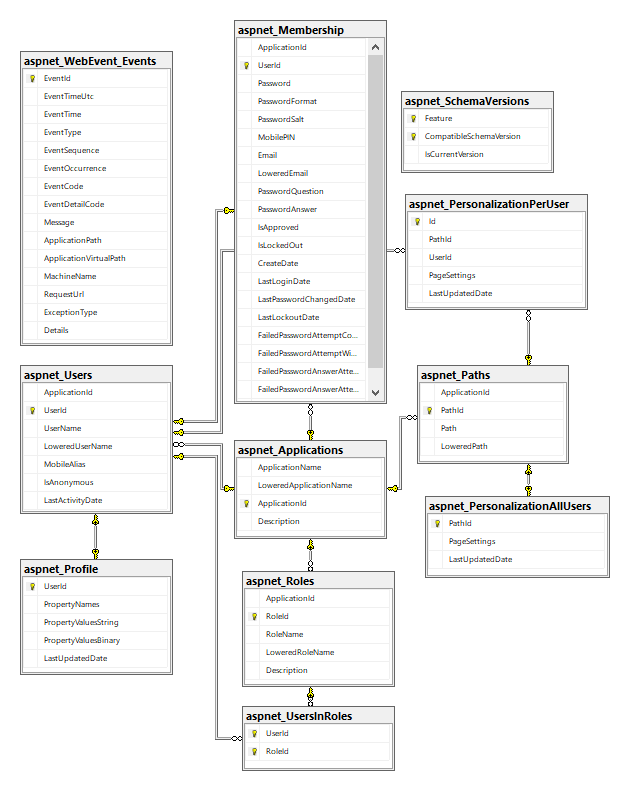
\includegraphics[width=1\linewidth]{schema.png}
    \caption{Sơ đồ ASP.NET Membership}
    \label{fig:schema}
\end{figure}

Cơ sở dữ liệu của hệ thống được thiết kế với cấu trúc phức tạp và logic, bao gồm nhiều bảng dữ liệu và mối quan hệ chặt chẽ giữa chúng. Hình ảnh \ref{fig:schema} minh họa rõ ràng cách các bảng dữ liệu chính liên kết với nhau, tạo nên một hệ thống cơ sở dữ liệu mạnh mẽ để hỗ trợ các chức năng cốt lõi của ứng dụng.

Bảng aspnet\_Users là trung tâm lưu trữ thông tin cơ bản về thành viên. Trong đó, cột UserId đóng vai trò là khóa chính, giúp định danh duy nhất từng thành viên. Các trường như UserName, MobileAlias, và LastActivityDate lưu trữ thông tin nhận diện và hoạt động của thành viên, hỗ trợ việc theo dõi và quản lý tài khoản.

Liên kết chặt chẽ với bảng này là aspnet\_Membership, nơi lưu trữ các thông tin liên quan đến bảo mật và trạng thái tài khoản thành viên. UserId trong bảng aspnet\_Membership là khóa ngoại, liên kết với aspnet\_Users, tạo ra mối quan hệ 1-1 giữa thông tin thành viên và thông tin thành viên. Các trường như Password, PasswordSalt, IsApproved, và LastLoginDate giúp quản lý quá trình xác thực và bảo mật tài khoản, đảm bảo rằng chỉ những thành viên hợp lệ mới có thể truy cập vào hệ thống.

aspnet\_Roles là bảng quản lý vai trò trong hệ thống. Mỗi vai trò được định danh bởi RoleId, và bảng này kết nối với aspnet\_Users thông qua bảng nối aspnet\_UsersInRoles. Bảng nối này sử dụng các khóa ngoại UserId và RoleId để thiết lập mối quan hệ nhiều-nhiều, cho phép một thành viên có thể đảm nhận nhiều vai trò khác nhau. Điều này mang lại sự linh hoạt trong việc phân quyền và quản lý thành viên.

Ngoài ra, aspnet\_Profile là bảng lưu trữ các thông tin tùy chỉnh và mở rộng về hồ sơ cá nhân của thành viên. Các trường PropertyNames, PropertyValuesString, và PropertyValuesBinary chứa các thông tin như sở thích cá nhân, cài đặt giao diện, và các thuộc tính cá nhân hóa khác. Bảng này giúp tạo ra trải nghiệm thành viên được cá nhân hóa trong hệ thống, nâng cao tính linh hoạt và sự tương tác với thành viên.

Bảng aspnet\_WebEvent\_Events theo dõi và ghi nhận các sự kiện xảy ra trong hệ thống, chẳng hạn như lỗi hệ thống, các hoạt động quan trọng, và các thay đổi trong ứng dụng. Bảng này lưu trữ các thông tin chi tiết về sự kiện, bao gồm thời gian xảy ra (EventTimeUtc), loại sự kiện (EventType), và thông báo sự kiện (Message). Thông tin này rất quan trọng cho việc giám sát và xử lý sự cố trong hệ thống, giúp đảm bảo hệ thống hoạt động ổn định và an toàn.

Các bảng aspnet\_Paths, aspnet\_PersonalizationPerUser, và aspnet\_PersonalizationAllUsers quản lý các cài đặt cá nhân hóa và đường dẫn trong hệ thống. aspnet\_Paths lưu trữ các thông tin về đường dẫn trong ứng dụng, trong khi hai bảng cá nhân hóa lưu trữ các thiết lập tùy chỉnh cho từng thành viên hoặc áp dụng chung cho tất cả thành viên. Sự phân tách này giúp hệ thống linh hoạt trong việc điều chỉnh nội dung và trải nghiệm dựa trên sở thích và hành vi của thành viên.

Cuối cùng, aspnet\_SchemaVersions giúp quản lý phiên bản của schema cơ sở dữ liệu, đảm bảo rằng hệ thống luôn đồng bộ với các cập nhật mới nhất. Bảng này lưu trữ các thông tin về các phiên bản schema, giúp duy trì tính toàn vẹn và nhất quán của cơ sở dữ liệu khi có thay đổi hoặc nâng cấp.

Cơ sở dữ liệu của hệ thống được thiết kế với cấu trúc chặt chẽ, bao gồm nhiều bảng dữ liệu và mối quan hệ giữa chúng. Tuy nhiên, trong phạm vi luận văn chỉtập trung chủ yếu vào 5 bảng chính: aspnet\_Membership, aspnet\_Profile, aspnet\_Roles, aspnet\_Users, và aspnet\_UsersInRoles. Những bảng này đóng vai trò cốt lõi trong việc quản lý thành viên, vai trò và các thông tin liên quan đến bảo mật và hồ sơ cá nhân trong hệ thống.



\subsubsection{Thiết lập hệ thống distributed database}

Để thiết lập một hệ thống cơ sở dữ liệu phân tán, bước đầu tiên là chuẩn bị môi trường phần cứng và phần mềm cần thiết. Mỗi node trong hệ thống cần có CPU đa nhân, RAM lớn và ổ đĩa SSD để đảm bảo hiệu suất cao. Hệ điều hành Linux, như CentOS hoặc Ubuntu, thường được sử dụng do tính ổn định và hiệu quả trong môi trường node. Các gói phần mềm cơ bản như SSH, rsync và các công cụ quản lý hệ thống khác cần được cài đặt trên mỗi node. Đối với mỗi hệ thống cụ thể, như Greenplum, CockroachDB, YugabyteDB và TiDB, có thể yêu cầu thêm các gói phần mềm và công cụ quản lý đặc thù.

Mạng nội bộ kết nối các node phải có tốc độ cao và ổn định để đảm bảo việc truyền tải dữ liệu nhanh chóng và giảm thiểu độ trễ. Các node cần có khả năng giao tiếp với nhau thông qua SSH không cần mật khẩu, điều này yêu cầu thiết lập các khóa SSH để xác thực không cần mật khẩu giữa các node. Điều này đảm bảo rằng các node có thể được quản lý từ xa một cách hiệu quả, tạo điều kiện cho việc cấu hình và triển khai hệ thống một cách dễ dàng và an toàn.

Việc lựa chọn phần mềm cơ sở dữ liệu phù hợp là rất quan trọng. Greenplum, CockroachDB, YugabyteDB và TiDB đều có những đặc điểm riêng biệt và ưu điểm cụ thể. Greenplum được thiết kế cho các tác vụ phân tích dữ liệu lớn nhờ kiến trúc MPP. CockroachDB và YugabyteDB nổi bật với tính nhất quán và khả năng chịu lỗi cao, trong khi TiDB cung cấp tính linh hoạt và khả năng tương thích cao với MySQL.

Quá trình cài đặt phần mềm bao gồm tải xuống và triển khai trên tất cả các node. Ví dụ, với Greenplum, cần thiết lập Master và Segment nodes. CockroachDB và YugabyteDB yêu cầu cài đặt và cấu hình các Replica nodes để đảm bảo tính sẵn sàng và độ chịu lỗi. TiDB đòi hỏi cài đặt các thành phần TiDB server, TiKV (key-value storage), và PD (Placement Driver) trên các node tương ứng. Đảm bảo rằng tất cả các node đều cài đặt cùng một phiên bản phần mềm để tránh xung đột trong quá trình vận hành.

Sau khi cài đặt, các tệp cấu hình của hệ thống cần được thiết lập để các node có thể hoạt động như một cụm đồng nhất. Đối với Greenplum, các tệp như pg\_hba.conf và postgresql.conf cần được cấu hình cẩn thận. CockroachDB sử dụng tệp cockroach.yaml để cấu hình các tham số hệ thống, YugabyteDB yêu cầu cấu hình trong yugabyted.conf, và TiDB sử dụng tidb.toml cùng với các cấu hình liên quan cho TiKV và PD. Các tệp cấu hình này xác định cách thức các node giao tiếp với nhau, cách dữ liệu được phân phối và các thông số khác liên quan đến hiệu suất và bảo mật.

Trong hệ thống Greenplum, các node được chia thành Master và Segment nodes, nơi Master node quản lý và điều phối các hoạt động. CockroachDB và YugabyteDB sử dụng mô hình phân tán ngang với các Replica nodes để đảm bảo tính sẵn sàng và độ chịu lỗi. TiDB cấu trúc thành các node TiDB server, TiKV và PD để phân chia nhiệm vụ quản lý và lưu trữ dữ liệu. Việc thiết lập các vai trò này giúp tối ưu hóa việc phân phối và quản lý dữ liệu trong hệ thống, đảm bảo rằng hệ thống có thể hoạt động một cách hiệu quả và ổn định.

Các công cụ phân phối dữ liệu tích hợp trong phần mềm cơ sở dữ liệu được sử dụng để phân chia dữ liệu giữa các node. Greenplum sử dụng kiến trúc MPP để phân phối dữ liệu và tải công việc giữa các Segment nodes. CockroachDB và YugabyteDB sử dụng các cơ chế phân phối dữ liệu đồng đều giữa các node để tối ưu hóa hiệu suất và đảm bảo tính nhất quán. TiDB phân chia dữ liệu thông qua TiKV, sử dụng các vùng (regions) để quản lý dữ liệu một cách hiệu quả. Các cơ chế này giúp tối ưu hóa hiệu suất và đảm bảo rằng hệ thống có thể xử lý tải công việc lớn một cách hiệu quả.

Sau khi cấu hình, cụm cơ sở dữ liệu được khởi tạo bằng cách khởi động tất cả các node và thiết lập kết nối giữa chúng. Quá trình khởi tạo này thiết lập kết nối giữa các node và xác nhận rằng cụm đang hoạt động chính xác. Ví dụ, khởi tạo cụm Greenplum yêu cầu khởi động Master và Segment nodes và thiết lập kết nối giữa chúng. CockroachDB và YugabyteDB yêu cầu khởi tạo cụm thông qua các lệnh cấu hình để thiết lập và liên kết các Replica nodes. TiDB yêu cầu khởi động và liên kết các thành phần TiDB server, TiKV và PD để đảm bảo hoạt động đồng bộ và hiệu quả của hệ thống.

Sau khi khởi tạo cụm, cần thực hiện kiểm tra tính toàn vẹn của hệ thống để đảm bảo rằng các node có thể giao tiếp với nhau một cách hiệu quả và dữ liệu được phân phối đúng cách. Sử dụng các công cụ giám sát tích hợp trong Greenplum, CockroachDB, YugabyteDB và TiDB để đánh giá hiệu suất và xác định các điểm cần tối ưu hóa. Các bài kiểm tra này nên bao gồm việc kiểm tra các truy vấn cơ bản, hiệu suất ghi và đọc dữ liệu, cũng như khả năng chịu lỗi của hệ thống.

Thiết lập hệ thống cơ sở dữ liệu phân tán là một quy trình phức tạp nhưng cần thiết để đảm bảo rằng hệ thống có thể đáp ứng các yêu cầu về hiệu suất và khả năng mở rộng trong quản lý dữ liệu lớn. Bằng cách tuân thủ các bước cài đặt và cấu hình chi tiết, có thể thiết lập một hệ thống cơ sở dữ liệu phân tán mạnh mẽ, linh hoạt và hiệu quả, đáp ứng tốt các nhu cầu của doanh nghiệp trong môi trường dữ liệu ngày càng phát triển. Sự chuẩn bị kỹ lưỡng, kiểm tra cẩn thận và tối ưu hóa liên tục sẽ giúp đảm bảo rằng hệ thống hoạt động một cách ổn định và hiệu quả, mang lại lợi ích tối đa cho tổ chức.

\subsubsection{Dữ liệu}

Trong quá trình chuyển đổi cơ sở dữ liệu ASP.NET Membership từ một hệ thống cơ sở dữ liệu tập trung như MSSQL sang một hệ thống cơ sở dữ liệu phân tán như Greenplum, CockroachDB, YugabyteDB, hoặc TiDB, việc chuyển dữ liệu là một trong những bước quan trọng và phức tạp nhất. Quy trình này bao gồm các bước kiểm tra dữ liệu, chuyển dữ liệu, chuyển đổi stored procedures (SPs), và kiểm thử. Dưới đây là một phân tích chi tiết về từng bước trong quy trình này.

Trước khi tiến hành chuyển đổi, cần thực hiện kiểm tra và đánh giá toàn diện dữ liệu hiện có trong cơ sở dữ liệu MSSQL. Việc này bao gồm kiểm tra tính toàn vẹn của dữ liệu, xác định các bảng, khóa ngoại, chỉ mục, và các stored procedures. Phân tích này giúp xác định các yêu cầu chuyển đổi cụ thể và đảm bảo rằng tất cả dữ liệu cần thiết sẽ được chuyển đổi một cách chính xác và đầy đủ.Đảm bảo rằng dữ liệu trong cơ sở dữ liệu hiện tại không bị lỗi hoặc thiếu sót là bước quan trọng để tránh các vấn đề tiềm ẩn trong quá trình chuyển đổi. Kiểm tra tính nhất quán của dữ liệu, bao gồm việc xác minh các ràng buộc toàn vẹn dữ liệu, khóa ngoại và các chỉ mục(index), giúp đảm bảo rằng dữ liệu sẽ được duy trì đúng như trong hệ thống mới.


Biến đổi dữ liệu trích xuất để phù hợp với cấu trúc và định dạng của hệ thống cơ sở dữ liệu phân tán mới. Quá trình biến đổi này bao gồm việc chuyển đổi kiểu dữ liệu, điều chỉnh các khóa ngoại và tối ưu hóa cấu trúc bảng. Sau khi biến đổi, dữ liệu được tải vào hệ thống cơ sở dữ liệu phân tán như Greenplum, CockroachDB, YugabyteDB, hoặc TiDB. Bước này đòi hỏi kiểm tra kỹ lưỡng để đảm bảo rằng dữ liệu được nhập chính xác và đầy đủ.

Các stored procedures trong cơ sở dữ liệu MSSQL cần được viết lại hoặc điều chỉnh để tương thích với hệ thống cơ sở dữ liệu phân tán mới. Do cú pháp và chức năng của stored procedures có thể khác nhau giữa các hệ thống cơ sở dữ liệu, cần đảm bảo rằng các stored procedures vẫn hoạt động đúng như mong đợi sau khi chuyển đổi. Ví dụ, stored procedures trong MSSQL cần được chuyển đổi để phù hợp với cú pháp của Greenplum hoặc CockroachDB.

Sau khi chuyển đổi, cần tiến hành kiểm thử toàn diện để đảm bảo rằng tất cả dữ liệu đã được chuyển đổi một cách chính xác và không có mất mát hoặc sai lệch. Sử dụng các công cụ kiểm thử dữ liệu để so sánh dữ liệu giữa hệ thống cũ và hệ thống mới, đảm bảo rằng dữ liệu trong hệ thống mới duy trì tính nhất quán và toàn vẹn.

\subsubsection{Kiểm tra hệ thống distributed database khi chuyển đổi}

Quá trình kiểm tra hệ thống cơ sở dữ liệu phân tán là một bước quan trọng nhằm đảm bảo rằng hệ thống hoạt động đúng như mong đợi về hiệu suất và khả năng mở rộng. Trong bối cảnh chuyển đổi từ ASP.NET Membership database sang các hệ thống phân tán như Greenplum, CockroachDB, YugabyteDB và TiDB, việc kiểm tra hệ thống bao gồm hai khía cạnh chính: hiệu suất (performance) và khả năng mở rộng (scale).

Trước khi chuyển đổi, cần ghi lại các chỉ số hiệu suất quan trọng của hệ thống cơ sở dữ liệu tập trung hiện tại. Các chỉ số này bao gồm thời gian phản hồi của truy vấn, tốc độ đọc/ghi dữ liệu, và tải hệ thống. Việc này giúp tạo ra một cơ sở so sánh để đánh giá hiệu suất của hệ thống cơ sở dữ liệu phân tán sau khi chuyển đổi.

Sau khi hoàn tất chuyển đổi sang hệ thống cơ sở dữ liệu phân tán, thực hiện kiểm thử hiệu suất toàn diện để đánh giá thời gian phản hồi và tốc độ xử lý của hệ thống mới. Các công cụ như Apache JMeter hoặc các công cụ kiểm thử tích hợp sẵn trong Greenplum, CockroachDB, YugabyteDB và TiDB có thể được sử dụng để thực hiện các bài kiểm tra này. Kiểm thử cần bao gồm các kịch bản tải cao và kiểm tra khả năng xử lý đồng thời để đảm bảo rằng hệ thống mới đáp ứng các yêu cầu hiệu suất.

So sánh các chỉ số hiệu suất sau khi chuyển đổi với các chỉ số hiệu suất trước khi chuyển đổi để xác định xem hệ thống cơ sở dữ liệu phân tán có cải thiện hiệu suất hay không. Điều này giúp xác định được những lợi ích cụ thể của việc chuyển đổi và đánh giá tính hiệu quả của hệ thống mới.

Một trong những ưu điểm lớn của hệ thống cơ sở dữ liệu phân tán là khả năng mở rộng theo chiều ngang (scale-out). Để kiểm tra khả năng này, cần thêm các node mới vào cụm cơ sở dữ liệu phân tán và đánh giá tác động của việc này lên hiệu suất hệ thống. Với Greenplum, việc bổ sung các segment node mới sẽ được thực hiện, trong khi CockroachDB và YugabyteDB yêu cầu thêm các replica node. TiDB yêu cầu thêm các TiKV nodes và kiểm tra sự phân phối lại dữ liệu.

Sau khi thêm các node mới, tiến hành các bài kiểm tra hiệu suất để đánh giá khả năng xử lý của hệ thống với cấu hình mở rộng. Các chỉ số như thời gian phản hồi, tốc độ đọc/ghi và tải hệ thống cần được đo lường và so sánh với cấu hình ban đầu để xác định hiệu quả của việc mở rộng.

Thực hiện các bài kiểm tra khả năng chịu tải để xác định hệ thống cơ sở dữ liệu phân tán có thể xử lý khối lượng công việc lớn đến mức nào mà không bị giảm hiệu suất. Điều này bao gồm việc mô phỏng các tình huống tải cao và đánh giá cách thức hệ thống phân tán quản lý và phân phối tải công việc giữa các node.

Một yếu tố quan trọng khác trong kiểm tra khả năng mở rộng là kiểm tra khả năng chịu lỗi của hệ thống. Điều này bao gồm việc mô phỏng các tình huống mất mát node và kiểm tra xem hệ thống có thể tự động phân phối lại tải công việc và duy trì tính nhất quán dữ liệu hay không. Các hệ thống như CockroachDB và YugabyteDB đặc biệt mạnh về khả năng này, nhờ vào thiết kế tập trung vào tính nhất quán và khả năng chịu lỗi.

Ngoài việc kiểm tra hiệu suất và khả năng mở rộng, việc kiểm tra tính chính xác của dữ liệu và các chức năng của hệ thống là một bước không thể thiếu. Điều này đặc biệt quan trọng trong quá trình chuyển đổi từ hệ thống cơ sở dữ liệu tập trung sang hệ thống cơ sở dữ liệu phân tán, nhằm đảm bảo rằng hệ thống mới không chỉ đáp ứng các yêu cầu về hiệu suất mà còn duy trì tính toàn vẹn và chính xác của dữ liệu.

Một trong những thành phần quan trọng của việc kiểm tra tính chính xác là giao diện người dùng. Các tính năng như đăng nhập và danh sách thành viên cần được kiểm tra kỹ lưỡng. Chức năng đăng nhập là một phần cốt lõi của bất kỳ hệ thống quản lý thành viên nào. Để kiểm tra chức năng này, cần sử dụng các tài khoản thành viên với các quyền hạn khác nhau để đăng nhập vào hệ thống. Việc kiểm tra này nhằm đảm bảo rằng hệ thống xử lý thông tin đăng nhập một cách chính xác, cho phép truy cập đối với thông tin hợp lệ và từ chối truy cập đối với thông tin không hợp lệ. Đây là bước quan trọng để xác nhận rằng hệ thống duy trì tính bảo mật và toàn vẹn sau khi chuyển đổi.

Chức năng hiển thị danh sách thành viên cũng phải được kiểm tra kỹ lưỡng để đảm bảo rằng tất cả thông tin thành viên được hiển thị đúng cách và không có sự mất mát dữ liệu. Việc kiểm tra này đảm bảo rằng dữ liệu người dùng không chỉ được duy trì mà còn có thể được truy xuất một cách hiệu quả trong hệ thống mới.

Bằng cách thực hiện các kiểm tra thủ công đối với các tính năng quan trọng như đăng nhập và danh sách thành viên, ta có thể xác minh rằng hệ thống hoạt động đúng như mong đợi cũng như đánh giá hiệu quả sau khi chuyển đổi. Điều này giúp đảm bảo rằng hệ thống cơ sở dữ liệu phân tán không chỉ đáp ứng các nhu cầu hiện tại mà còn sẵn sàng cho các yêu cầu phát triển trong tương lai. Việc kiểm tra toàn diện này là yếu tố then chốt để đảm bảo sự thành công của quá trình chuyển đổi và tối ưu hóa hoạt động của hệ thống trong môi trường mới.

\subsection{Lựa chọn Greenplum thay thế MSSQL.}

Nhận thức được những thách thức trong việc quản lý và xử lý dữ liệu lớn, giải pháp đề xuất trong luận văn này là áp dụng Greenplum. Việc lựa chọn Greenplum để chuyển đổi cơ sở dữ liệu ASP.NET Membership từ MSSQL sang môi trường phân tán là một quyết định có cơ sở và được cân nhắc kỹ lưỡng dựa trên nhiều yếu tố then chốt. Dưới đây là những lý do chính khiến Greenplum nổi bật và trở thành lựa chọn tốt hơn so với các giải pháp thay thế như TiDB, CockroachDB và YugabyteDB:

\textbf{Kiến trúc MPP tối ưu hóa cho phân tích dữ liệu.}

Greenplum, với kiến trúc xử lý song song mạnh mẽ MPP, được thiết kế đặc biệt để xử lý khối lượng dữ liệu lớn và các truy vấn phân tích phức tạp. Kiến trúc MPP của Greenplum cho phép phân phối khối lượng công việc trên nhiều node, giúp tối ưu hóa hiệu suất xử lý và giảm thời gian truy vấn. Điều này đặc biệt phù hợp với nhu cầu phân tích và báo cáo về dữ liệu người dùng trong hệ thống Membership, nơi yêu cầu các truy vấn phức tạp và khối lượng dữ liệu lớn. So với CockroachDB và YugabyteDB, vốn chủ yếu tập trung vào tính khả dụng cao và tính nhất quán, Greenplum vượt trội trong việc tối ưu hóa cho các tác vụ phân tích dữ liệu lớn.

\textbf{Tương thích SQL toàn diện.}

Greenplum cung cấp hỗ trợ toàn diện cho các tiêu chuẩn SQL, điều này làm cho việc chuyển đổi dữ liệu và ứng dụng từ MSSQL trở nên trơn tru và ít rủi ro hơn. Khả năng tương thích SQL của Greenplum cho phép các nhà phát triển tiếp tục sử dụng các câu lệnh SQL quen thuộc, từ đó giảm thiểu đáng kể công sức và thời gian cần thiết cho quá trình chuyển đổi so với việc phải học các ngôn ngữ truy vấn mới như trong TiDB\footnote{\url{https://docs.pingcap.com/tidb/stable/mysql-compatibility}}. Hơn nữa, Greenplum hỗ trợ các giao thức kết nối chuẩn như ODBC, JDBC và các công cụ trích xuất, biến đổi và tải dữ liệu (Extract, Transform, Load - ETL) phổ biến. Điều này giúp dễ dàng tích hợp với các công cụ và ứng dụng hiện có, chẳng hạn như Tableau, Power BI, và Talend. Khả năng tích hợp này đảm bảo rằng các quy trình hiện tại có thể tiếp tục mà không cần thay đổi lớn.

Tính tương thích SQL toàn diện của Greenplum còn giúp dễ dàng tích hợp với các công cụ và ứng dụng hiện có, điều mà các giải pháp như CockroachDB và YugabyteDB, với sự tập trung vào tính nhất quán phân tán, có thể không hỗ trợ một cách hoàn hảo. Nhờ vào sự hỗ trợ mạnh mẽ này, Greenplum không chỉ đảm bảo sự chuyển đổi liền mạch mà còn giúp duy trì hiệu suất và tính ổn định của hệ thống trong suốt quá trình chuyển đổi.


\textbf{Khả năng mở rộng linh hoạt.}

Greenplum không chỉ hỗ trợ mở rộng theo chiều ngang (scale-out) mà còn thể hiện khả năng vượt trội trong việc thích ứng linh hoạt với sự gia tăng quy mô hệ thống. Việc bổ sung các node mới vào hệ thống được thực hiện một cách liền mạch, không gây gián đoạn đến hoạt động của các node hiện có, đảm bảo tính liên tục và ổn định của dịch vụ.

Cơ chế phân phối dữ liệu thông minh của Greenplum đóng vai trò then chốt trong việc duy trì hiệu suất tối ưu khi hệ thống mở rộng. Cơ chế này tự động phân bổ dữ liệu một cách cân bằng trên toàn bộ các node trong hệ thống. Khi thêm node mới, Greenplum tự động điều chỉnh lại việc phân phối dữ liệu, từ đó tối ưu hóa hiệu suất truy vấn và đảm bảo tải được phân bổ đồng đều trên toàn bộ hệ thống. Điều này giúp duy trì hiệu năng ổn định và đảm bảo rằng các tài nguyên được sử dụng một cách hiệu quả nhất.

Khả năng mở rộng của Greenplum đã được kiểm chứng qua nhiều triển khai thực tế trong các hệ thống lớn và phức tạp. Các doanh nghiệp đã sử dụng Greenplum để xử lý khối lượng dữ liệu khổng lồ và các yêu cầu tính toán cao, chứng minh rằng hệ thống có thể duy trì hiệu năng mạnh mẽ ngay cả khi đối mặt với sự tăng trưởng dữ liệu đột biến. Điều này đặc biệt quan trọng trong bối cảnh hiện nay, khi mà dữ liệu lớn ngày càng trở nên phổ biến và yêu cầu xử lý dữ liệu trong thời gian thực ngày càng cao.

So sánh với các giải pháp khác như TiDB và CockroachDB, Greenplum không chỉ hỗ trợ mở rộng theo chiều ngang mà còn nổi bật với khả năng mở rộng vượt trội về mặt hiệu suất và tính ổn định. Trong khi TiDB và CockroachDB tập trung vào tính nhất quán phân tán và khả năng mở rộng, Greenplum đem lại một sự kết hợp hoàn hảo giữa khả năng mở rộng, hiệu năng xử lý và sự linh hoạt trong quản lý dữ liệu. Khả năng này giúp Greenplum đáp ứng tốt hơn các yêu cầu khắt khe của các hệ thống doanh nghiệp, nơi mà hiệu suất và tính ổn định là những yếu tố quan trọng hàng đầu.

Khả năng thích ứng và mở rộng của Greenplum không chỉ đảm bảo rằng hệ thống có thể phát triển cùng với nhu cầu kinh doanh mà còn giúp giảm thiểu các rủi ro liên quan đến gián đoạn dịch vụ. Việc mở rộng hệ thống được thực hiện mà không cần phải tạm dừng hoặc ảnh hưởng đến hoạt động hiện tại, điều này cực kỳ quan trọng trong các môi trường kinh doanh yêu cầu tính liên tục cao.

Greenplum cung cấp một nền tảng mạnh mẽ cho các hệ thống cơ sở dữ liệu phân tán, không chỉ đáp ứng mà còn vượt qua các yêu cầu về khả năng mở rộng và hiệu suất. Với cơ chế phân phối dữ liệu thông minh và khả năng mở rộng linh hoạt, Greenplum chứng minh mình là lựa chọn lý tưởng cho các doanh nghiệp cần một hệ thống cơ sở dữ liệu mạnh mẽ, ổn định và có khả năng mở rộng cao.



\textbf{Hiệu suất vượt trội trong xử lý truy vấn phức tạp.}

Nhờ vào kiến trúc MPP và khả năng tối ưu hóa truy vấn mạnh mẽ, Greenplum thể hiện hiệu suất vượt trội trong việc xử lý các truy vấn phân tích phức tạp trên dữ liệu Membership. Kiến trúc MPP của Greenplum cho phép hệ thống phân chia công việc xử lý truy vấn thành nhiều phần nhỏ và thực hiện chúng song song trên nhiều node, từ đó tối ưu hóa tốc độ xử lý và giảm thiểu thời gian phản hồi.

Greenplum sử dụng các thuật toán tối ưu hóa tiên tiến để tăng tốc độ truy vấn và xử lý dữ liệu. Các thuật toán này bao gồm tối ưu hóa kế hoạch thực thi truy vấn, quản lý bộ nhớ hiệu quả, và sử dụng các cấu trúc dữ liệu tiên tiến để tăng cường hiệu suất. Nhờ đó, Greenplum có thể xử lý một khối lượng lớn dữ liệu và các truy vấn phức tạp một cách hiệu quả, đặc biệt trong các môi trường yêu cầu phân tích dữ liệu lớn.

So với TiDB, vốn có thể gặp khó khăn trong việc xử lý các truy vấn phức tạp, Greenplum vượt trội về hiệu suất xử lý truy vấn. TiDB, mặc dù mạnh mẽ trong việc duy trì tính nhất quán và khả năng chịu lỗi, nhưng có thể bị hạn chế khi phải xử lý các truy vấn đòi hỏi nhiều tài nguyên và tính toán phức tạp. Trong khi đó, Greenplum được thiết kế để tối ưu hóa cho các tác vụ phân tích, với khả năng xử lý hàng loạt dữ liệu lớn và các truy vấn phân tích đa chiều một cách nhanh chóng và hiệu quả.

Hiệu suất vượt trội của Greenplum đảm bảo rằng hệ thống có thể đáp ứng nhanh chóng các yêu cầu phân tích và báo cáo. Điều này đặc biệt quan trọng trong các hệ thống quản lý thành viên trực tuyến như ASP.NET Membership, nơi mà việc phân tích và báo cáo dữ liệu người dùng một cách nhanh chóng và chính xác là vô cùng cần thiết. Khả năng xử lý các truy vấn phức tạp một cách hiệu quả giúp Greenplum hỗ trợ tốt hơn cho các quyết định kinh doanh dựa trên dữ liệu và cải thiện trải nghiệm người dùng cuối.

Tóm lại, nhờ vào kiến trúc MPP và các thuật toán tối ưu hóa tiên tiến, Greenplum không chỉ đảm bảo hiệu suất vượt trội trong việc xử lý các truy vấn phân tích phức tạp mà còn cung cấp một nền tảng mạnh mẽ và linh hoạt cho các nhu cầu phân tích dữ liệu lớn. Điều này làm cho Greenplum trở thành lựa chọn lý tưởng cho các doanh nghiệp cần một hệ thống cơ sở dữ liệu mạnh mẽ, ổn định và có khả năng đáp ứng cao.



\textbf{Tích hợp với hệ sinh thái dữ liệu lớn.}

Greenplum không chỉ cung cấp khả năng xử lý và phân tích dữ liệu mạnh mẽ mà còn dễ dàng tích hợp với các hệ sinh thái dữ liệu lớn như Hadoop, Spark và Kafka. Khả năng tích hợp này tạo ra một nền tảng toàn diện và linh hoạt, cho phép xử lý và phân tích dữ liệu lớn một cách hiệu quả. Nhờ vào khả năng tích hợp liền mạch với Hadoop, Greenplum có thể tận dụng sức mạnh của hệ thống phân tán này để lưu trữ và xử lý dữ liệu không giới hạn. Việc tích hợp với Spark giúp tăng cường khả năng xử lý dữ liệu nhanh chóng và phân tích theo thời gian thực, trong khi Kafka cung cấp khả năng quản lý luồng dữ liệu liên tục và đáng tin cậy giữa các hệ thống.

Khả năng tích hợp mạnh mẽ này là một điểm khác biệt quan trọng của Greenplum so với các giải pháp khác như CockroachDB và YugabyteDB. Mặc dù CockroachDB và YugabyteDB cũng hỗ trợ các tính năng phân tán và nhất quán, nhưng khả năng tích hợp với các hệ sinh thái dữ liệu lớn của chúng có thể không toàn diện và linh hoạt như Greenplum. Greenplum hỗ trợ các giao thức chuẩn và công cụ tích hợp, cho phép hệ thống hoạt động một cách trơn tru trong các môi trường dữ liệu phức tạp và đa dạng.

Việc tích hợp với Hadoop, Spark và Kafka giúp Greenplum không chỉ xử lý các tác vụ lưu trữ và phân tích dữ liệu lớn mà còn hỗ trợ quản lý và điều phối luồng dữ liệu liên tục giữa các hệ thống. Điều này rất quan trọng trong các môi trường doanh nghiệp hiện đại, nơi dữ liệu được thu thập từ nhiều nguồn khác nhau và cần được xử lý và phân tích một cách nhanh chóng và chính xác.

Khả năng tích hợp toàn diện của Greenplum với các hệ sinh thái dữ liệu lớn như Hadoop, Spark và Kafka không chỉ tạo ra một nền tảng mạnh mẽ để xử lý và phân tích dữ liệu lớn mà còn làm nổi bật sự linh hoạt và khả năng mở rộng của hệ thống. Điều này giúp Greenplum vượt trội so với các giải pháp khác và trở thành lựa chọn hàng đầu cho các môi trường dữ liệu phức tạp và đa dạng.

Nhờ vào khả năng tích hợp mạnh mẽ và linh hoạt, Greenplum trở thành một lựa chọn lý tưởng cho các doanh nghiệp cần một hệ thống cơ sở dữ liệu có khả năng mở rộng, hiệu suất cao và dễ dàng tích hợp với các công cụ và hệ sinh thái dữ liệu lớn hiện có. Điều này giúp doanh nghiệp tận dụng tối đa giá trị của dữ liệu, hỗ trợ ra quyết định nhanh chóng và chính xác, và đáp ứng hiệu quả các yêu cầu kinh doanh ngày càng phức tạp.
